\section{Leistungsfluss über eine Leitung}
\subsubsection{Mathematische Vereinfachungen im Voraus}
    \begin{minipage}[c]{0.48\columnwidth}
            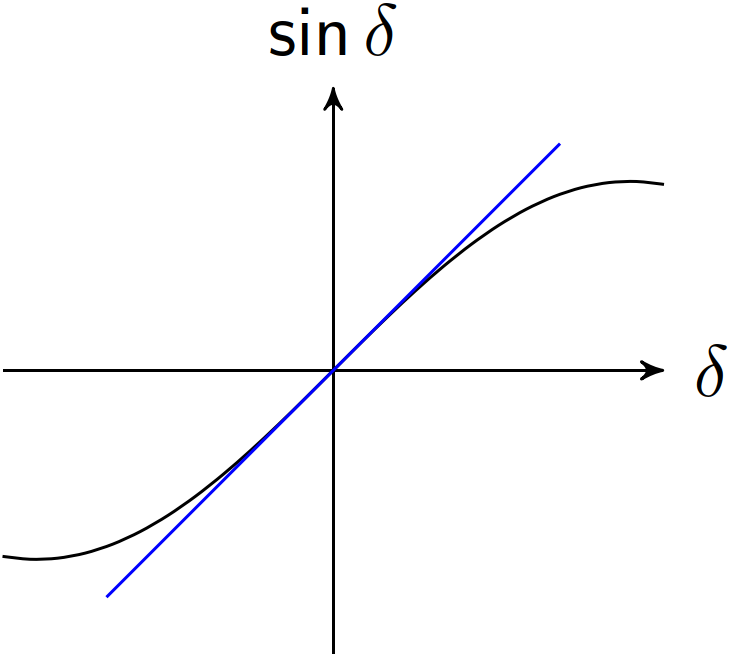
\includegraphics[width=0.7\textwidth, align=c]{images/Erkenntnisse_1.png}

            \begin{itemize}
                \item für kleinere Winkel: $\sin\delta \approx \delta$
                \item Maximale Steigung
            \end{itemize}    
    \end{minipage}
    \hfill
    \begin{minipage}[c]{0.48\columnwidth}
            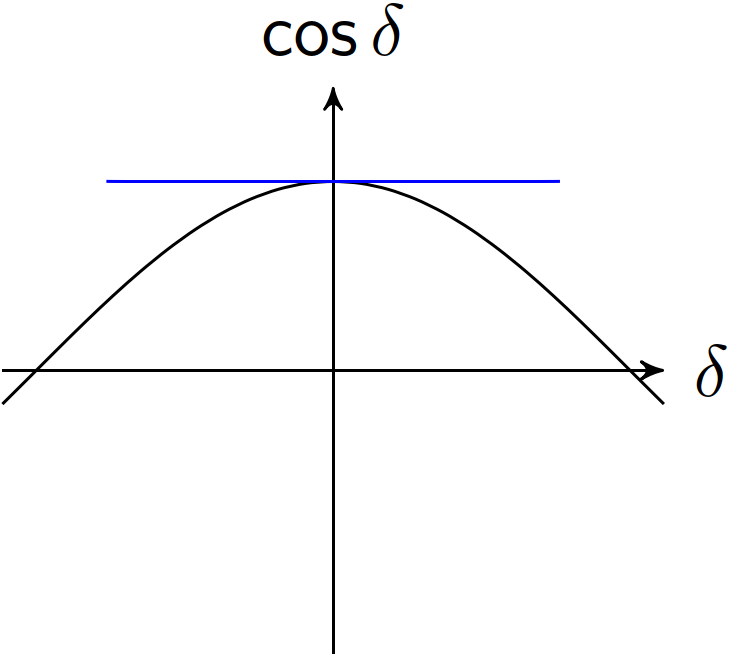
\includegraphics[width=0.7\textwidth, align=c]{images/Erkenntnisse_2.png}

            \begin{itemize}
                \item für kleinere Winkel: $\cos\delta \approx 1$
                \item Minimale Steigung
            \end{itemize}
    \end{minipage}

\subsection{Leistungsfluss}
    \begin{minipage}[t]{0.6\columnwidth}
        \centering \vspace{-0.7\baselineskip}
        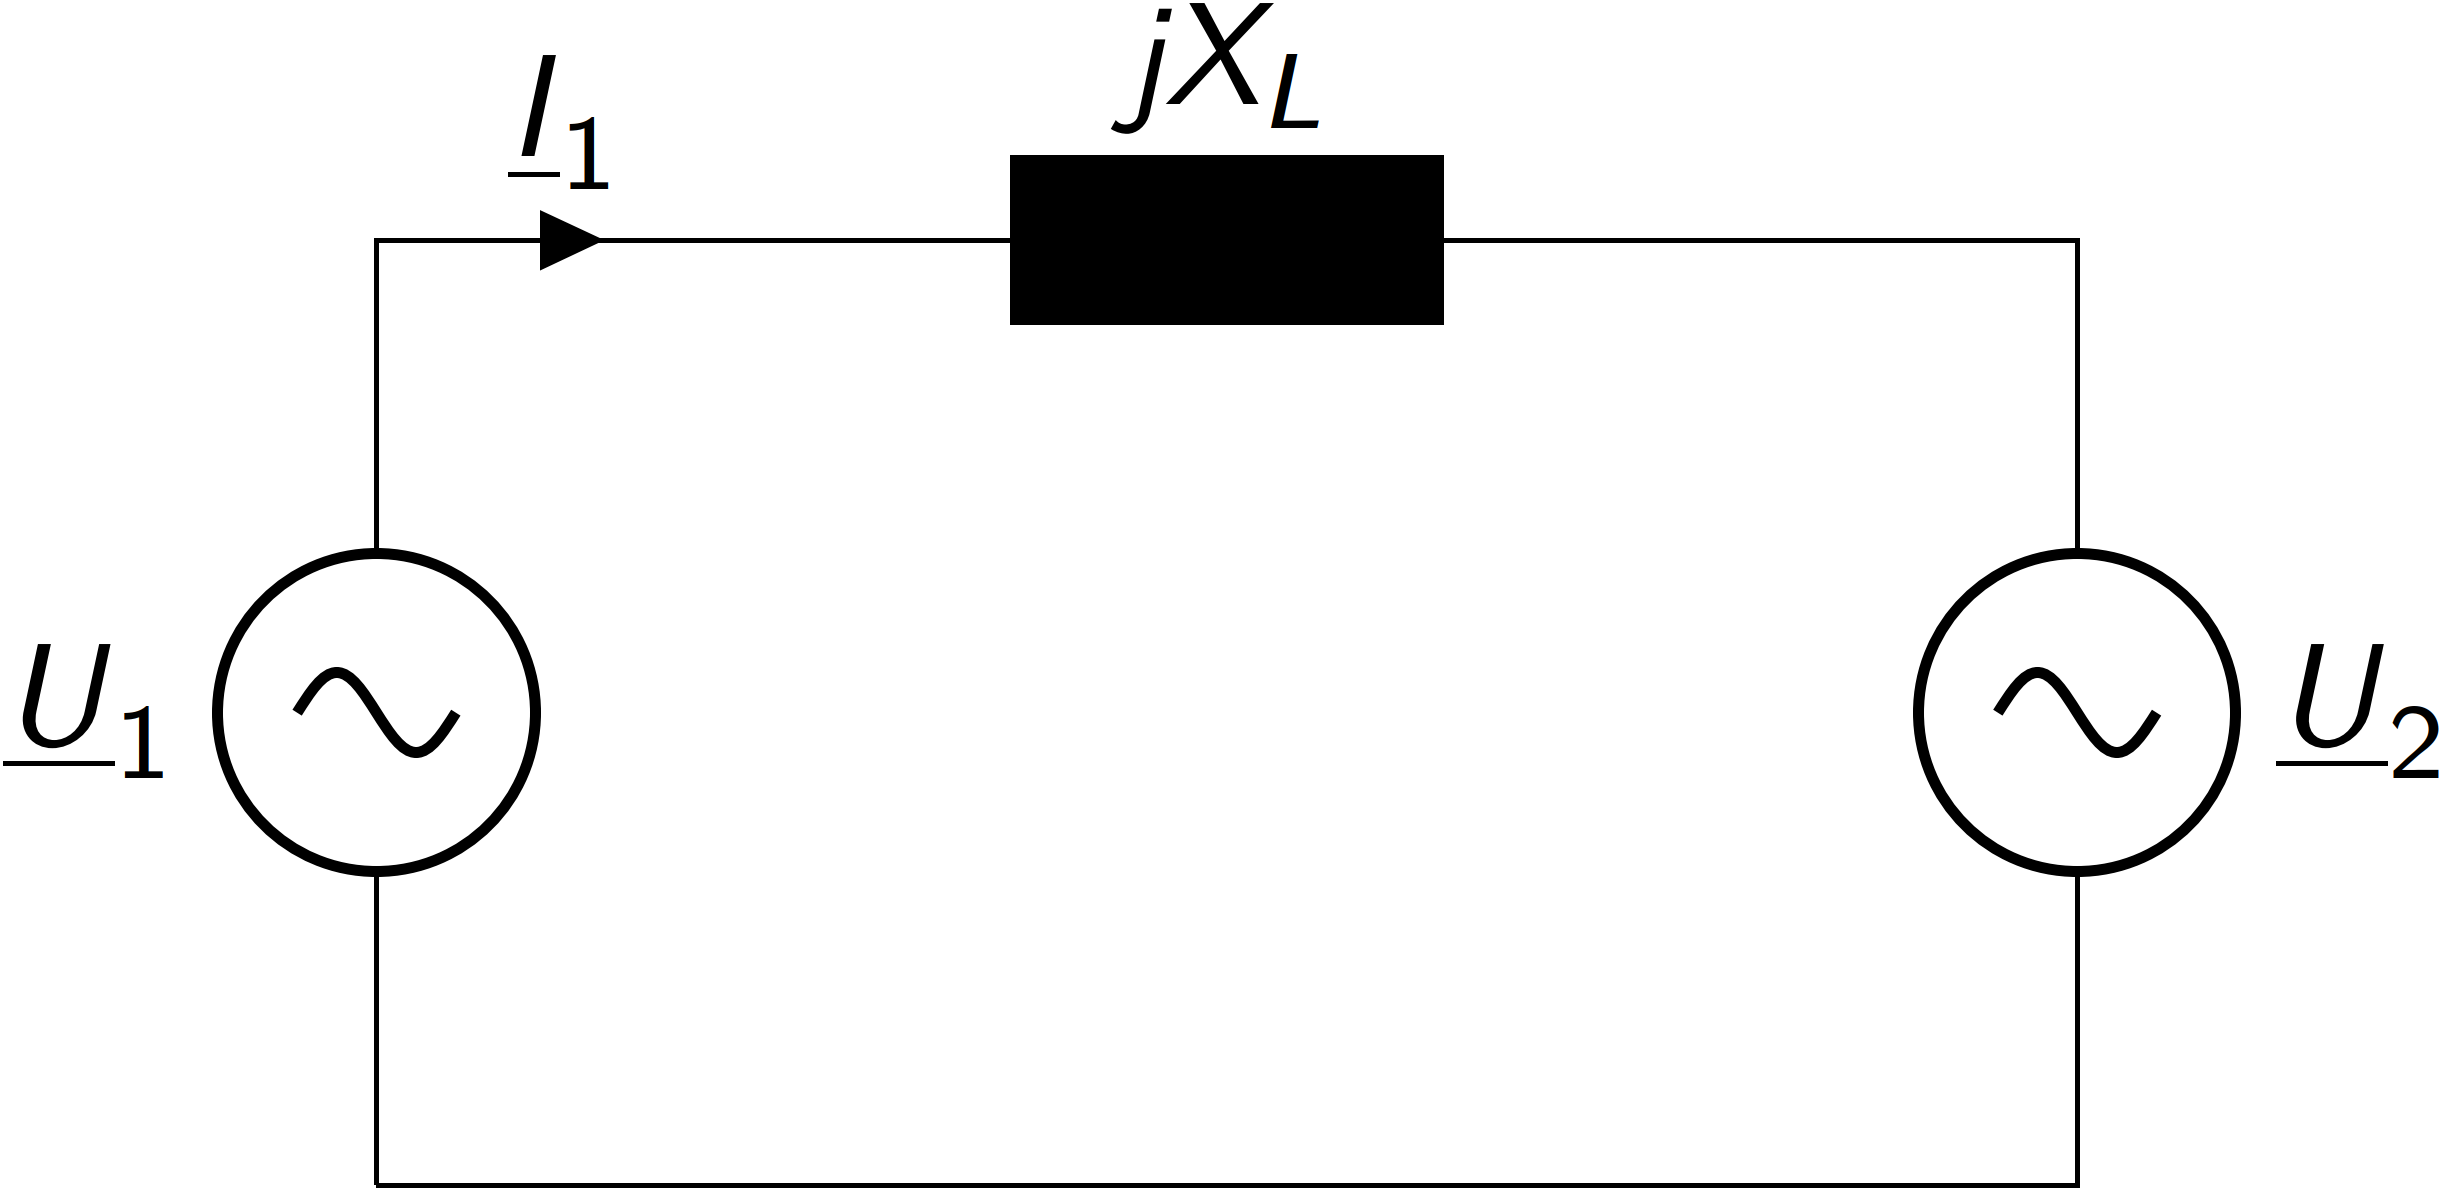
\includegraphics[width=0.85\linewidth]{images/Leistungsübertragung_1.png}
    \end{minipage}%
    \hfill
    \begin{minipage}[t]{0.39\columnwidth}
        \begin{itemize}
            \item Verlustlose Leitung
            \item Ideale Spannungsquellen $\underline{U}_1$ und $\underline{U}_2$
        \end{itemize}
    \end{minipage}

\subsection{Leistungsübertragung}
    $\boxed{\underline{U}_1 = U_1 \cdot e^{j \cdot \theta_1}} \quad \boxed{\underline{U}_2 = U_2 \cdot e^{j \cdot \theta_2}}$
    $\quad$
    $\boxed{X_L = \omega \cdot L = \omega \cdot L' \cdot l} \quad \boxed{\omega = 2 \cdot \pi \cdot f}$

    \vspace{0.1cm}

    % $\boxed{\underline{I}_1 = \frac{U_1 - U_2}{j \cdot X_L} = \frac{U_1 \cdot e^{j \cdot \theta_1} - U_2 \cdot e^{j \cdot \theta_2}}{j \cdot X_L}} \quad $

    $\boxed{\underline{I}_1^* = \frac{U_1 \cdot e^{-j \cdot \theta_1} - U_2 \cdot e^{-j \cdot \theta_2}}{-j \cdot X_L}
    = \frac{j}{X_L} \left( U_1 \cdot e^{-j \cdot \theta_1} - U_2 \cdot e^{-j \cdot \theta_2} \right)}$

    \vspace{0.1cm}

    $\boxed{\delta = \theta_1 - \theta_2}$
    $\boxed{\underline{S}_1 = \underline{U}_1 \cdot \underline{I}_1^* = {P}_1 + j \cdot {Q}_1}$

    $\boxed{
    \underline{S}_1 = \underbrace{U_1 \cdot U_2 \cdot \frac{1}{X_L} \cdot \sin(\delta)}_{P_1}
    + j\, \underbrace{\left( U_1^2 \cdot \frac{1}{X_L} - U_1 \cdot U_2 \cdot \frac{1}{X_L} \cos(\delta) \right)}_{Q_1}}$

    \vspace{0.1cm}

    $\boxed{P_1 = \text{Re}\left\{ \underline{U}_1 \cdot \underline{I}_1^*\right\}= U_1 \cdot U_2 \cdot \frac{1}{X_L} \cdot \sin(\delta)}$

    \vspace{0.1cm}

    $\boxed{Q_1 = \text{Im}\left\{ \underline{U}_1 \cdot \underline{I}_1^*\right\} = U_1^2 \cdot \frac{1}{X_L} - U_1 \cdot U_2 \cdot \frac{1}{X_L} \cos(\delta)}$

    \renewcommand{\arraystretch}{1.2}
    \begin{tabular}{@{} l p{6cm} l @{}}
    $U_1$        & Effektive Spannungen am Leitungsanfang \dotfill & $\mathrm{V}$ \\
    $U_2$        & Effektive Spannungen am Leitungsende \dotfill & $\mathrm{V}$ \\
    $\theta_1$ & Phasenwinkel der Spannungen am Leitungsanfang \dotfill & $\mathrm{rad}$ \\
    $\theta_2$ & Phasenwinkel der Spannungen am Leitungsende \dotfill & $\mathrm{rad}$ \\
    % $j$                 & Imaginäre Einheit ($j^2 = -1$) \dotfill & $-$ \\
    $\omega$            & Kreisfrequenz \dotfill & $\mathrm{rad/s}$ \\
    $f$                 & Netzfrequenz \dotfill & $\mathrm{Hz}$ \\
    $L$                 & Induktivität der Leitung \dotfill & $\mathrm{H}$ \\
    $L'$                & Induktivität pro Längeneinheit \dotfill & $\mathrm{H/m}$ \\
    $l$                 & Leitungslänge \dotfill & $\mathrm{m}$ \\
    $X_L$               & Reaktanz der Leitung  \dotfill & $\Omega$ \\
    % $I_1$               & Strom am Leitungsanfang \dotfill & $\mathrm{A}$ \\
    $I_1^*$             & Komplex konjugierter Strom \dotfill & $\mathrm{A}$ \\
    $S_1$               & Scheinleistung am Leitungsanfang \dotfill & $\mathrm{VA}$ \\
    $P_1$               & Wirkleistung \dotfill & $\mathrm{W}$ \\
    $Q_1$               & Blindleistung \dotfill & $\mathrm{VAR}$ \\
    $\delta$           & Phasendifferenz \dotfill & $\mathrm{rad}$ \\
    \end{tabular}

\subsection{Praxis (Vereinfachung)}\label{Leistungsübertragung}
    $U_1 \approx U_2$, $\delta$ in der Regel klein, $\delta \leq 40^\circ$

    % \vspace{0.1cm}
    Mit den Vereinfachungen (Anfangs Kapitel) und den aufgeführten Punkten ergibt sich:
    % \vspace{0.1cm}

    $\boxed{P_{12} = \frac{U_1 U_2}{X} \sin(\delta_{12})}$
    $\boxed{Q_{12} = \frac{U_1^2 - U_1 U_2 \cdot \cos(\delta_{12})}{X}}$
    $\boxed{Q_{21} = \frac{U_2^2 - U_2 U_1 \cdot \cos(-\delta_{12})}{X}}$

\subsubsection{Erkenntisse für Wirk- und Blindleistung}
    \begin{minipage}[t]{0.49\columnwidth}
        \textbf{Wirkleistung:}

        \begin{itemize}
            \item \textbf{Stark} abh. von der Phasendifferenz $\delta$
            \item \textbf{Wenig} abh. vom Spannungsbetrag $U_1, U_2$
        \end{itemize}
    \end{minipage}%
    \hfill
    \begin{minipage}[t]{0.49\columnwidth}
        \textbf{Blindleistung:}

        \begin{itemize}
            \item \textbf{Stark} abh. von der Phasendifferenz $\delta$
            \item \textbf{Wenig} abh. vom Spannungsbetrag $U_1, U_2$
        \end{itemize}
    \end{minipage}

\subsection{Maximale Wirkleistungsübertragung}
    \begin{minipage}[c]{0.35\columnwidth}
        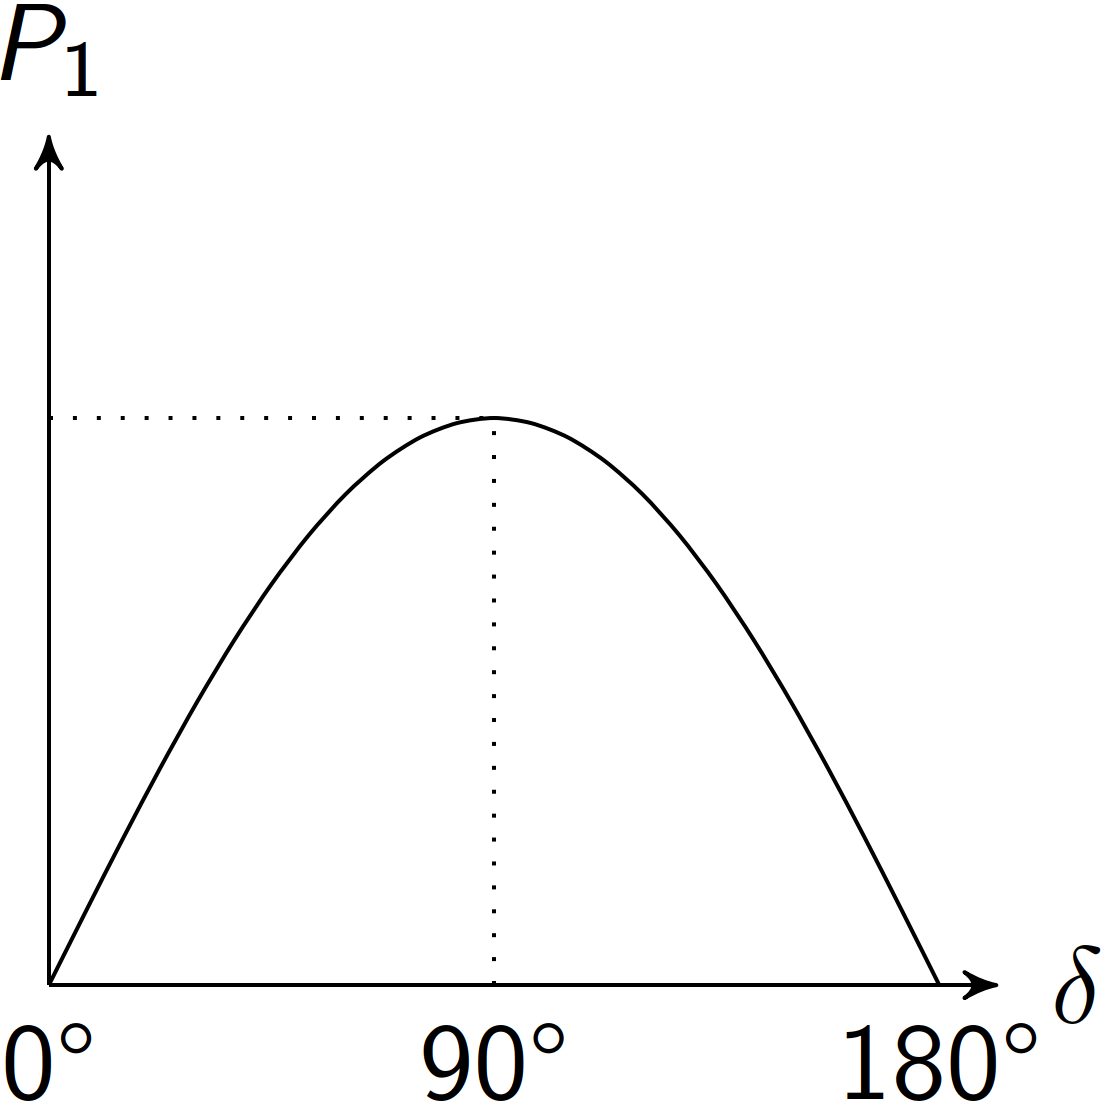
\includegraphics[width=0.7\textwidth]{images/Maximale_Wirkleistungsübertragung.png}
    \end{minipage}
    \hfill
    \begin{minipage}[c]{0.48\columnwidth}
        $\boxed{P_{1_{\text{max}}}^{1ph} = \frac{U_1 \cdot U_2}{X_{12}}}$

        $\boxed{P_{1_{\text{max}}} = 3\frac{U_1 \cdot U_2}{X_{12}}}$
    \end{minipage}